% ============================================================
% PDIG-D-26-00342 v5 (Major Revision, Option A reframe) -- revised main manuscript
% Built on the PLOS template scaffold (plos2015). v5 for finalization. Markers:
%   [SEED] = value to be replaced with seeded canonical output from make (repro gate)
%   [VBIB] = verify against the real v4 .bib at finalization
%   [SBSENS] = insert Systemic-Bias 10-barrier sensitivity result
% ============================================================
\documentclass[10pt,letterpaper]{article}
\usepackage[top=0.85in,left=2.75in,footskip=0.75in]{geometry}
\usepackage{amsmath,amssymb,amsthm}
\usepackage{changepage}
\usepackage{textcomp,marvosym}
\usepackage{cite}
\usepackage{nameref,hyperref}
\usepackage[right]{lineno}
\usepackage{silence}
\WarningFilter{latex}{Command \showhyphens has changed}
\usepackage[nopatch=eqnum]{microtype}
\DisableLigatures[f]{encoding = *, family = * }
\usepackage[table]{xcolor}
\usepackage{array}
\usepackage{float}
\usepackage{placeins} % provides \FloatBarrier to control float placement

\newcolumntype{+}{!{\vrule width 2pt}}
\newlength\savedwidth
\newcommand\thickcline[1]{\noalign{\global\savedwidth\arrayrulewidth\global\arrayrulewidth 2pt}\cline{#1}\noalign{\vskip\arrayrulewidth}\noalign{\global\arrayrulewidth\savedwidth}}
\newcommand\thickhline{\noalign{\global\savedwidth\arrayrulewidth\global\arrayrulewidth 2pt}\hline\noalign{\global\arrayrulewidth\savedwidth}}

\raggedright
\setlength{\parindent}{0.5cm}
\textwidth 5.25in
\textheight 8.75in
\usepackage[aboveskip=1pt,labelfont=bf,labelsep=period,justification=raggedright,singlelinecheck=off]{caption}
\renewcommand{\figurename}{Fig}
\bibliographystyle{plos2015}
\makeatletter
\renewcommand{\@biblabel}[1]{\quad#1.}
\makeatother
\usepackage{lastpage,fancyhdr,graphicx}
\graphicspath{{figures/}{../manuscript/figures/}}
\usepackage{epstopdf}
\pagestyle{fancy}
\fancyhf{}
\rfoot{\thepage/\pageref{LastPage}}
\renewcommand{\headrulewidth}{0pt}
\renewcommand{\footrule}{\hrule height 2pt \vspace{2mm}}
\fancyheadoffset[L]{2.25in}
\fancyfootoffset[L]{2.25in}
\lfoot{\today}

\newtheorem{proposition}{Proposition}

\begin{document}
\vspace*{0.2in}

% ============================================================
% TITLE
% ============================================================
\begin{flushleft}
{\Large
\textbf\newline{Structural limits of single-barrier reform in algorithmic recourse: a formal series-system model with implications for digital health}
}
\newline
\\
A.C.\ Demidont,\ DO\textsuperscript{1,*}
\\
\bigskip
\textbf{1} Independent Researcher, Nyx Dynamics, LLC, Philadelphia, Pennsylvania, United States of America
\\
\bigskip
* acdemidont@nyxdynamics.org
\end{flushleft}

% ============================================================
% ABSTRACT
% ============================================================
\section*{Abstract}
Algorithmic decision systems mediate access to healthcare, credit, employment, and housing, and individuals who receive adverse decisions must pass through multiple sequential barriers to obtain recourse. We develop a \emph{formal series-system model} in which successful recourse requires passage through 11 stages across three layers (data integration, data accuracy, institutional access), and we analyze its structural properties. We prove two results: single-barrier interventions are algebraically bounded by baseline system success (Proposition~1), and probability-scale multiplicativity necessarily generates higher-order interaction terms (Proposition~2). Parameterizing the model with pass probabilities mapped from federal datasets and one healthcare algorithmic audit---a mapping we treat as provisional and transport-limited---the baseline recourse probability is 0.0018\% and no single-barrier removal exceeds 0.0054\%. A factorial decomposition attributes 87.6\% of achievable improvement to the three-way cross-layer interaction; Shapley attribution, Sobol and Morris sensitivity analyses, and bootstrap resampling illustrate this structure within prespecified perturbation ranges. Relaxing the independence assumption with a Gaussian-copula analysis (correlation up to $\rho=0.5$) leaves the comparative conclusion---single-layer reform yields far less than coordinated reform---intact, while a repeated-attempt topology attenuates it, delimiting the model's domain of validity. These findings are properties of the modeled system rather than empirical measurements of real recourse pathways; they yield testable hypotheses for digital-health governance---chiefly, that fairness interventions confined to a single layer are structurally unlikely to produce large absolute gains---that remain to be validated against observed recourse data.

\linenumbers

% ============================================================
% INTRODUCTION
% ============================================================
\section*{Introduction}
Algorithmic systems increasingly mediate access to fundamental opportunities across domains. Employment-screening tools filter a large majority of applicants before human review~\cite{bib_fuller,bib_eeoc,bib_ajunwa,bib_raghavan}; credit-scoring systems shape access to housing, insurance, and finance~\cite{bib_cfpb_credit}; and healthcare algorithms allocate resources and prioritize interventions across populations~\cite{bib_obermeyer}. When such systems produce adverse decisions, affected individuals must seek \emph{recourse}---error detection, data correction, and institutional appeal---across processes that are often technically and institutionally fragmented.

Recourse from adverse algorithmic decisions has been studied largely as a per-decision, per-model problem (for example, actionable recourse~\cite{bib_ustun} and counterfactual explanations~\cite{bib_wachter}), and fairness is increasingly understood as a property of the surrounding sociotechnical system~\cite{bib_selbst}. Yet obtaining recourse in practice requires navigating a \emph{sequence} of administrative and technical barriers, any one of which can block resolution. Series-structured systems of this kind are well characterized in reliability engineering, where overall performance is dominated by interactions among components rather than by any single element~\cite{bib_rausand,bib_billinton}, and in patient-safety analysis, where adverse events arise from the alignment of multiple latent failures~\cite{bib_reason}.

We ask a structural question: \emph{in a multi-stage barrier system governing recourse from adverse algorithmic decisions, under what conditions do single-barrier reforms have negligible absolute impact, and how much of the achievable improvement is attributable to cross-layer interactions?} We formalize recourse as an 11-stage series system, prove closed-form bounds on single-barrier effects, and quantify the interaction structure by factorial decomposition, Shapley attribution, and global sensitivity analysis. Healthcare is our motivating application and the setting for the digital-health implications we draw; credit, employment, and housing are co-equal domains from which most parameters are, in fact, sourced. We are explicit throughout that our numerical results are properties of the model under a specific parameterization, not empirical measurements of how any real recourse system behaves.

% ============================================================
% METHODS
% ============================================================
\section*{Materials and methods}

\subsection*{Scope of claims: framework, formal model, calibration, and hypotheses}
To prevent conflation of model properties with empirical findings, we distinguish four levels of claim and use them consistently. \textbf{(1) Theorem-level results} are mathematical consequences that hold given the model (Propositions~1--2). \textbf{(2) Numerical/model illustrations} are simulation or decomposition outputs generated from the chosen topology and parameterization (the 0.0018\% baseline, the 0.0054\% maximum single-barrier gain, the 87.6\% three-way share, and the Shapley/Sobol/Morris/bootstrap outputs); these are \emph{consistent with}, not independent confirmation of, the propositions, because both derive from the same multiplicative structure. \textbf{(3) Empirical calibration assumptions} are the 11 pass probabilities mapped from heterogeneous federal, legal, administrative, and healthcare sources; these are provisional and transport-limited. \textbf{(4) Real-system claims}---statements about actual recourse behavior or policy effectiveness---are treated as hypotheses pending validation against observed recourse trajectories.

\subsection*{Barrier model specification}
We model successful recourse as requiring passage through 11 sequential barriers organized into three layers (Table~\ref{table1}). Layer~1 (Data Integration): Rapid Data Transmission ($p=0.30$), Multi-System Integration ($p=0.55$), Permanent Storage ($p=0.45$). Layer~2 (Data Accuracy): Error Detection Difficulty ($p=0.35$), Correction Process Barriers ($p=0.35$), Incomplete Correction Propagation ($p=0.40$). Layer~3 (Institutional): Awareness Gap ($p=0.30$), Record Access Barriers ($p=0.55$), Legal Knowledge Gap ($p=0.25$), Legal Resource Barriers ($p=0.40$), Systemic Bias in Algorithms ($p=0.30$).

\begin{table}[htbp]
\centering
\caption{{\bf Barrier parameters and layer assignments.} Pass probabilities and empirically bounded ranges are derived in Supplementary Table~S-Deriv; ten of the eleven parameters derive from cross-domain (credit/dispute/legal) sources, and one (Systemic Bias) from a healthcare audit.}
\label{table1}
\begin{tabular}{l l c}
\hline
\textbf{Layer} & \textbf{Barrier} & \textbf{Pass prob.} \\
\thickhline
Data Integration & Rapid Data Transmission & 0.30 \\
 & Multi-System Integration & 0.55 \\
 & Permanent Storage & 0.45 \\ \hline
Data Accuracy & Error Detection Difficulty & 0.35 \\
 & Correction Process Barriers & 0.35 \\
 & Incomplete Correction Propagation & 0.40 \\ \hline
Institutional & Awareness Gap & 0.30 \\
 & Record Access Barriers & 0.55 \\
 & Legal Knowledge Gap & 0.25 \\
 & Legal Resource Barriers & 0.40 \\
 & Systemic Bias in Algorithms & 0.30 \\
\hline
\end{tabular}
\end{table}

\emph{Operational definition of successful recourse.} We define successful recourse as full end-to-end resolution: the underlying data are corrected, the adverse decision is reversed, and the correction propagates across the relevant institutions. This is a stringent endpoint, and it is itself a modeling choice: less stringent endpoints (for example, correction at a single institution) would raise the baseline. We adopt the stringent definition because partial resolution that does not propagate typically leaves the adverse decision effective downstream.

\subsection*{Mathematical framework}
Under the series model, the probability of successful recourse is
\begin{equation}
P(\text{success}) = \prod_{i=1}^{11} p_i .
\end{equation}
Writing the cascade as a product does \emph{not} assume statistical independence: by the chain rule, $P(S_1,\dots,S_n)=P(S_1)\prod_{i=2}^{n}P(S_i\mid S_1,\dots,S_{i-1})$, so the $p_i$ are properly understood as stage-specific \emph{conditional} pass probabilities. Our calibration (below) substitutes largely \emph{marginal/proxy} statistics for these conditionals; we test the consequences of that substitution explicitly (see ``Structural assumptions'').

\begin{proposition}[Single-barrier improvement bound]
Removing barrier $j$ (setting $p_j=1$) yields $\Delta_j = P\,(1/p_j - 1)$, where $P$ is the baseline success probability. The absolute improvement is therefore linear in $P$; when $P$ is small, every $\Delta_j$ is necessarily small regardless of which barrier is targeted. This is an algebraic property of series systems, not a simulation finding.
\end{proposition}

\begin{proposition}[Higher-order interaction under probability-scale multiplicativity]
Let $L_k=\prod_{i\in k}p_i$ be layer-aggregate probabilities, so $P=L_1L_2L_3$. On the probability scale, factorial contrasts of $P$ generate nonzero higher-order (including three-way) interaction terms, whereas on the log scale $\log P=\sum_i\log p_i$ is additive and interactions vanish. The \emph{existence} of higher-order interaction is thus a structural feature of probability-scale multiplicativity; its \emph{magnitude} (e.g., a specific three-way share) is parameterization- and topology-dependent and is not a universal property.
\end{proposition}

\noindent(Proposition~2 is deliberately stated as the existence of higher-order interaction rather than ``interaction dominance''; the 87.6\% share reported below is a level-2 numerical result, not a theorem.)

\subsection*{Structural assumptions: why a serial topology, and what changes if it is wrong}
The series/all-required topology and the use of marginal proxies for conditional pass probabilities are the model's principal structural assumptions, and---as Reviewer feedback rightly emphasized---the interaction structure is partly a consequence of them. We therefore (i) justify the serial abstraction (recourse requires \emph{all} of detection, correction, propagation, and institutional action to succeed; the abstraction is conservative, favoring higher pass probabilities), and (ii) test two plausible alternative topologies:
\begin{itemize}
\item \textbf{Correlated barriers (Gaussian copula).} We couple the 11 Bernoulli pass-events through a Gaussian copula with equicorrelation $\rho$ (and a within-layer ``block'' variant), sweeping $\rho\in[0,0.5]$ ($n=100{,}000$, seed 42), preserving each marginal $p_i$.
\item \textbf{Repeated attempts.} We allow $m$ independent opportunities to clear each stage, $p_i^{(m)}=1-(1-p_i)^m$, for $m=1,2,3$.
\end{itemize}
For each we report baseline success, maximum single-stage effect, the factorial three-way interaction share, and the comparative (single-layer vs.\ coordinated) conclusion.

\subsection*{Shapley attribution and global sensitivity}
We attribute system effect to individual barriers by Shapley decomposition~\cite{bib_shapley}. We conduct one-at-a-time ($\pm10\%$) sensitivity, Sobol global sensitivity indices~\cite{bib_sobol} with Saltelli sampling, Morris screening~\cite{bib_morris}, and bootstrap resampling; all barrier probabilities are additionally perturbed across $\pm33\%$ and across the empirically bounded ranges in Table~\ref{table1}/S-Deriv. All stochastic analyses are seeded (\texttt{default\_rng(42)}) and reproducible.

\subsection*{Empirical parameter derivation and transportability}
Pass probabilities were mapped from publicly available federal datasets (CFPB~\cite{bib_cfpb_credit,bib_cfpb_disputes,bib_cfpb_complaints}, FTC~\cite{bib_ftc}), Legal Services Corporation reports~\cite{bib_lsc}, and one healthcare algorithmic audit~\cite{bib_obermeyer}, using explicit derivation logic. Ten of the eleven parameters derive from cross-domain (credit/dispute/legal) sources; only the Systemic Bias parameter derives from a healthcare audit. Full per-barrier derivation---source, exact statistic (with page/table), mapping rule, resulting $p_i$, plausibility range, and \emph{transportability limitation}---is given in Supplementary Table~S-Deriv and mirrored in the repository (\texttt{data/parameter\_sources/parameter\_derivation.md}). Because most parameters are transported from non-healthcare settings, we treat the healthcare-specific interpretation as provisional.

\subsection*{Software and reproducibility}
Analyses were conducted in Python 3.10+ (NumPy, SciPy, Matplotlib). All results, tables, and figures are regenerated by a single \texttt{make} pipeline with pinned seed 42 and regression tests on the deterministic invariants; code and data are at \url{https://github.com/Nyx-Dynamics/algorithmic-bias-epidemiology-academic} and archived at Zenodo (DOI:10.5281/zenodo.22312977).

\subsection*{Use of artificial intelligence}
AI-assisted tools were used for literature-search support and language refinement; all analyses, interpretation, and conclusions are the author's. [Minor 8: exact model versions/dates to be confirmed from contemporaneous records; where a version cannot be documented, the tool and role are stated without an unverified version.]

% ============================================================
% RESULTS
% ============================================================
\section*{Results}

\subsection*{Baseline system characteristics}
The 11-barrier model yields a baseline success probability of 0.0018\% (level~2), i.e., fewer than 2 in 100{,}000 modeled individuals complete all barriers under the calibrated parameters.

\subsection*{Single-barrier effects}
Consistent with Proposition~1, removing any single barrier while others remain produces negligible absolute improvement: all individual effects are $<$0.02\%, the maximum being Legal Knowledge Gap removal ($\Delta=0.0054\%$), matching the analytic bound $P(1/0.25-1)$ (Fig~\ref{fig1}).

\subsection*{Strategy comparison (descriptive)}
Forward, backward, greedy, and random barrier-removal strategies all exhibit threshold (``hockey-stick'') trajectories, with near-zero improvement until the final barriers are removed (Fig~\ref{fig2}). We report this as a descriptive observation---all strategies converge only at near-complete removal---and have removed the previously reported strategy-equivalence ANOVA, which lacked a defensible sampling model.

\subsection*{Layer interaction structure}
A factorial decomposition (Table~\ref{table2}) attributes 87.6\% of achievable improvement to the three-way cross-layer interaction (level~2). Main effects are minimal (L1 0.02\%, L2 0.03\%, L3 0.36\%); among pairwise terms, Data Accuracy $\times$ Institutional is largest (7.03\%), followed by Data Integration $\times$ Institutional (4.51\%) and Data Integration $\times$ Data Accuracy (0.44\%). (This corrects a stale main-text table in the prior version whose pairwise values disagreed with the supplement, figure, and code.) We describe 87.6\% as a \emph{share of achievable improvement} from a baseline-relative factorial decomposition; it is distinct from, and not contradicted by, the smaller Sobol total-minus-first-order gaps reported below, which quantify within-range parameter perturbation rather than whole-layer removal.

\begin{table}[htbp]
\centering
\caption{{\bf Baseline-relative factorial decomposition of achievable improvement.} Values match the code, the Fig~\ref{fig3} heatmap, and the supplement; they correct a stale main-text table in the prior submission whose pairwise values were inconsistent with the figure and code.}
\label{table2}
\begin{tabular}{l c}
\hline
\textbf{Effect} & \textbf{Share of achievable improvement (\%)} \\
\thickhline
L1 (Data Integration) & 0.02 \\
L2 (Data Accuracy) & 0.03 \\
L3 (Institutional) & 0.36 \\ \hline
L1 $\times$ L2 & 0.44 \\
L1 $\times$ L3 & 4.51 \\
L2 $\times$ L3 & 7.03 \\ \hline
L1 $\times$ L2 $\times$ L3 (three-way) & 87.60 \\ \thickhline
Total & 100.0 \\
\hline
\end{tabular}
\end{table}

\subsection*{Robustness to alternative topologies}
Relaxing independence via the Gaussian copula, the baseline success probability is correlation-sensitive, rising from 0.0018\% toward the weakest barrier ($p=0.25$) as correlation increases (to 3.2\% at $\rho=0.5$). However, the three-way interaction share remains high (77--88\% across $\rho\in[0,0.5]$), and single-lever reform remains far weaker than coordinated reform: at $\rho=0.5$, the best single-layer intervention yields 4.5\% versus 96.8\% for coordinated removal. Under a repeated-attempt topology the strong conclusion attenuates---the three-way share falls to 53\% at $m=2$ and 25\% at $m=3$ as the baseline rises---indicating that the strong quantitative conclusions hold for approximately single-pass serial recourse and weaken if recourse is substantially iterative (Fig~\ref{fig6}). We interpret this as delimiting the model's domain of validity rather than as invalidating it.

\subsection*{Global sensitivity}
Total-order Sobol indices exceeded first-order indices for all barriers---modestly for some (Awareness Gap 0.112 vs.\ 0.109; Legal Knowledge Gap 0.111 vs.\ 0.110) and more clearly for others (Fig~\ref{fig4}). Morris screening identified Legal Knowledge Gap and Systemic Bias as having the highest interaction involvement.

\subsection*{Shapley attribution}
Shapley decomposition (seeded, seed 42) assigns comparatively even contributions across barriers---no single barrier exceeds $\sim$11\%---with the top contributors (Legal Knowledge Gap, Rapid Data Transmission, Systemic Bias in Algorithms, Incomplete Correction Propagation, Awareness Gap) spanning all three layers, consistent with cross-layer, interaction-driven structure rather than any single dominant barrier.

\subsection*{Systemic-Bias placement sensitivity}
Because ``Systemic Bias in Algorithms'' arguably reflects upstream generation of the adverse decision rather than a recourse-stage barrier, we re-ran the model with this barrier removed/reclassified (10-barrier variant). The qualitative conclusions are unchanged: baseline success rises from 0.0018\% to 0.0060\% (still far below 1\%), the three-way interaction share remains dominant (86.6\% vs.\ 87.6\%), and the maximum single-barrier effect remains below 0.02\% (0.0180\%, Legal Knowledge Gap). We therefore retain the barrier in the recourse cascade, while noting that its most natural interpretation is the persistence of bias during recourse rather than the generation of the initial adverse decision, and that the results do not depend on this choice.

\subsection*{Robustness to parameter uncertainty}
Findings are stable within the prespecified $\pm10$--$33\%$ perturbation ranges. We note, however, that the coefficient of variation of the output rises steeply with noise---to roughly 110\% at 25\% and 129\% at 30\% multiplicative noise (seeded values; because the output magnitude is very small and right-skewed, this coefficient is itself sampling-sensitive)---so robustness is claimed only within these bounded scenarios, not under arbitrary real-world uncertainty (Fig~\ref{fig5}). [Finalization note: these seeded values replace the previously reported unseeded 73.2\%/93.8\%, which the reviewer cited; the seeded run is if anything less robust.]

% ============================================================
% DISCUSSION
% ============================================================
\section*{Discussion}
Under a series-structured model of algorithmic recourse with cross-domain calibration, single-barrier reforms are algebraically bounded to small absolute effects when baseline success is low (Proposition~1), and probability-scale multiplicativity generates higher-order interaction terms (Proposition~2). The numerical results---0.0018\% baseline, 0.0054\% maximum single-barrier gain, an 87.6\% three-way interaction share, and threshold removal dynamics---are properties of the modeled system, not empirical measurements of real recourse. Their practical reading is a hypothesis: \emph{if} recourse behaves like a low-baseline serial barrier system, single-layer fairness interventions are unlikely to produce large absolute gains, and coordinated multi-layer intervention is required.

Our robustness analysis sharpens which parts of this picture are structural. The comparative/threshold conclusion (single-layer $\ll$ coordinated) is robust to substantial cross-barrier correlation; the specific baseline value and the 87.6\% point estimate are not, and the conclusion weakens if recourse permits repeated attempts. The appropriate domain of validity is therefore approximately single-pass, serial recourse with low baseline success; iterative or parallel recourse would require re-estimation.

\emph{On the healthcare interpretation.} The empirical foundation most often cited for algorithmic bias in healthcare, Obermeyer et al.~\cite{bib_obermeyer}, is a single audit of one widely used commercial risk-prediction algorithm applied to one health system. The bias arose from a specific design choice---predicting health-care \emph{cost} as a proxy for health \emph{need}---so that Black patients at a given risk score were sicker and under-referred; correcting it would raise the share of Black patients flagged for additional help from 17.7\% to 46.5\%. This is compelling but context-specific and cannot, on its own, calibrate ``healthcare algorithmic bias'' at population scale; we accordingly treat it as one motivating example rather than an empirical anchor. (We note that a prior version mischaracterized this study's magnitude as ``$\sim$62\% undertriage''; that figure is not supported by Obermeyer et al.\ and has been corrected.)

Healthcare-AI fairness research has matured since 2019 beyond single-algorithm cost-proxy audits: chest-radiograph classifiers systematically underdiagnose under-served subgroups~\cite{bib_seyyed}; models can recover self-reported race from medical images through latent pathways clinicians cannot detect~\cite{bib_gichoya}; and dataset-standard and reporting frameworks have emerged to address such harms~\cite{bib_arora,bib_alderman,bib_hoche}. Algorithmic bias in healthcare is thus multi-mechanism and modality-spanning, and our single-parameter healthcare calibration should be read in that light.

\emph{Governance implications (as hypotheses).} If the serial-barrier structure approximates real recourse, then fairness interventions confined to the algorithmic layer---bias mitigation or audit mandates alone---would be expected to have limited population-level effect without simultaneous attention to data-integration and institutional-access barriers. The regulatory fragmentation across agencies (CFPB, EEOC, HHS) mirrors the barrier fragmentation in the model and may impede the coordinated response the analysis suggests. These are testable implications, not demonstrated policy facts; validating them requires longitudinal, individual-level recourse data.

\emph{Limitations.} The model is a formal abstraction and does not observe individual recourse trajectories. Parameters are transported from heterogeneous, largely non-healthcare sources and substitute marginal for conditional probabilities. The simulation results derive from the same multiplicative structure as the propositions and are illustrative, not independent validation. Robustness holds within bounded perturbation scenarios, not arbitrary uncertainty. Future work should estimate conditional stage-transition probabilities from longitudinal administrative and clinical data and re-test the structure against observed recourse outcomes.

% ============================================================
% CONCLUSIONS
% ============================================================
\section*{Conclusions}
As a formal series-system model, algorithmic recourse exhibits structurally bounded single-barrier effects and interaction-driven improvement. Whether real recourse systems behave this way is an empirical question the model is designed to motivate, not to settle; if they do, effective mitigation would require coordinated, multi-layer intervention rather than isolated single-layer reform.
% ============================================================
% FIGURE LEGENDS (interpretive; see Minor 6)
% ============================================================
\FloatBarrier
\clearpage
\section*{Figures}
\begin{figure}[!htbp]\centering


\includegraphics[width=\linewidth]{individual_barrier_effects.png}
\caption{{\bf Single-barrier removal effects are structurally small.} Marginal effect of removing each barrier while others remain; all $<$0.02\%, with the maximum (Legal Knowledge Gap, 0.0054\%) matching the Proposition~1 bound. Practically, no single reform materially raises end-to-end recourse when baseline success is low. Error bars: 95\% bootstrap CI (seeded).}
\label{fig1}\end{figure}

\begin{figure}[p]\centering

\includegraphics[width=\linewidth]{stepwise_comparison.png}
\caption{{\bf Only near-complete barrier removal helps.} Forward, backward, greedy, and random removal strategies all show threshold trajectories; improvement is negligible until the final barriers fall (descriptive; no inferential test).}
\label{fig2}\end{figure}

\begin{figure}[p]\centering

\includegraphics[width=\linewidth]{interaction_heatmap.png}
\caption{{\bf Improvement is cross-layer.} Main effects (diagonal) are minimal; the largest pairwise term is Data Accuracy $\times$ Institutional; the three-way interaction (87.6\%, not shown) dominates achievable improvement.}
\label{fig3}\end{figure}

\begin{figure}[p]\centering

\includegraphics[width=\linewidth]{sensitivity_analysis.png}
\caption{{\bf Global sensitivity.} OAT sensitivity radar; Sobol first-order ($S_1$) and total-order ($S_T$) indices with 95\% CI (total exceeds first-order for all barriers, modestly for several); Morris $\mu^*$ vs.\ $\sigma$; and per-barrier interaction contribution ($S_T-S_1$).}
\label{fig4}\end{figure}

\begin{figure}[p]\centering

\includegraphics[width=\linewidth]{snr_robustness.png}
\caption{{\bf Robustness is bounded.} Signal-to-noise ratio vs.\ parameter noise; output uncertainty propagation; key-finding stability under $\pm10\%$ perturbation; and coefficient of variation rising to $\sim$110\% at 25\% and $\sim$129\% at 30\% noise (seeded), indicating robustness only within bounded scenarios.}
\label{fig5}\end{figure}

\begin{figure}[p]\centering
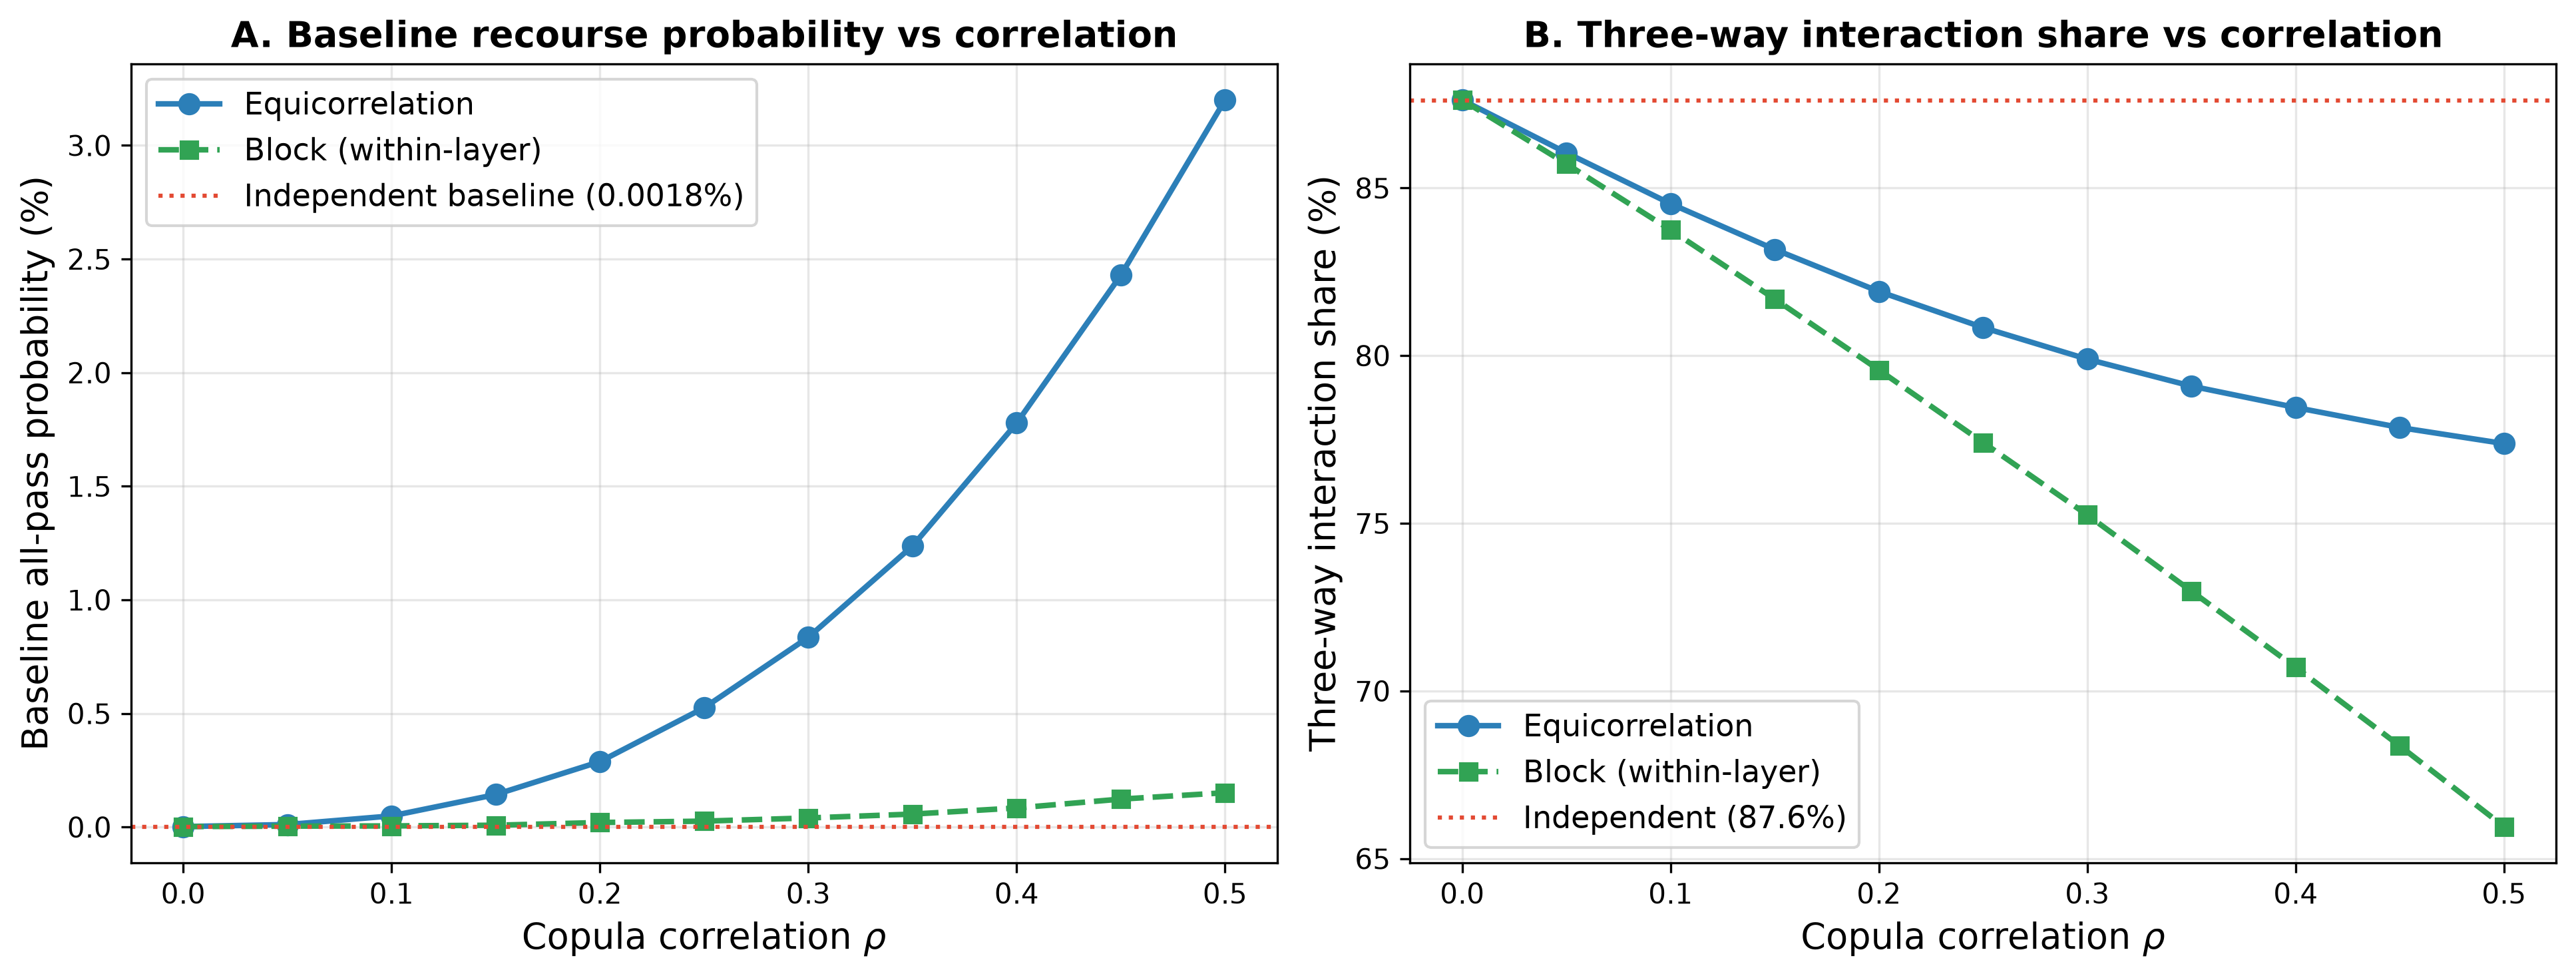
\includegraphics[width=\linewidth]{FigX_copula_robustness.png}
\caption{{\bf Alternative topologies delimit the model's validity.} Baseline success $P$ and three-way interaction share vs.\ Gaussian-copula correlation $\rho$ (the comparative conclusion is robust; the baseline value is correlation-sensitive), with repeated-attempt points ($m=2,3$) showing attenuation of interaction dominance under iterative recourse.}
\label{fig6}\end{figure}

\FloatBarrier
\clearpage
% ============================================================
% STANDARD SECTIONS
% ============================================================
\section*{Data availability}
All data and code are archived at Zenodo (DOI:10.5281/zenodo.22312977) and available at \url{https://github.com/Nyx-Dynamics/algorithmic-bias-epidemiology-academic}. A one-command \texttt{make} pipeline reproduces all results, tables, and figures (seed 42).

\section*{Ethics statement}
This study used publicly available, aggregate datasets and published statistics. No individual-level data were collected and no human subjects were enrolled; IRB approval was not required.

\section*{Competing interests}
A.C.D.\ reports prior employment with Gilead Sciences (January 2020--November 2024) and prior stock ownership fully divested December 2024; Gilead had no role in this study. A.C.D.\ owns Nyx Dynamics LLC. This research was conducted independently and not as part of any paid engagement. No other competing interests are declared.

\section*{Funding}
This work received no external funding.

\nolinenumbers
% ============================================================
% REFERENCES -- from references.bib (bibtex + plos2015.bst)
% ============================================================
\FloatBarrier
\clearpage
\bibliography{references}

\end{document}
